% !TEX root = ../masterthesis.tex
\chapter{Quantum Dot}

\section{Processing}

\section{Properties of our dots}

\begin{figure}[H]
	\centering
	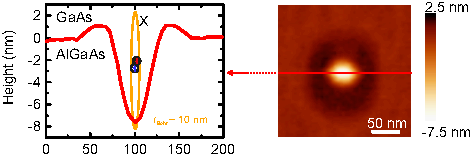
\includegraphics[width=0.9\linewidth]{figures/quantum-dot/QD_plot_AFM}
	\caption{Height profile (red) of a droplet-etched nanohole in an AlGaAs layer is shown in the left image.
	The orange line represents the wavefunction of the exciton which resembles the ground state of an hydrogen atom.
	Because of that the bohr radius $r_{\textrm{Bohr}}$ is denoted.
	The right image shows the atomic force microscopy picture of the nanohole.
	An GaAs quantum dot is obtained after filling the hole with GaAs and avergrowth with AlGaAs~\cite{reindl_highly_2019}}
	\label{fig:qdplotafm}
\end{figure}


\subsection{Calculate spectral range of zero-phonon line}
A typical lifetime of a GaAs quantum dot is $\Delta t = 250~ps$.
According to the time-energy uncertainty relation
\begin{align}
\Delta E \cdot \Delta t = \frac{h}{2 \pi}\\
\Rightarrow \Delta E = \SI{2.64}{\micro \electronvolt}
\end{align}
The frequency uncertainty can be obtained through
\begin{equation}
\Delta \nu = \frac{\Delta E}{h}
\end{equation}
By developing $\lambda$into a taylor series
\begin{align}
\label{eq:planck-einstein}
\lambda &= \frac{c}{\nu}\\
\Rightarrow \lambda(\nu) &\approx \lambda(\nu_0) + \lambda'(\nu_0) \cdot (\nu - \nu_0)
\end{align}
$\Delta \lambda$ can be expressed as
\begin{align}
\Delta \lambda &= \lambda(\nu_0 - \Delta \nu) - \lambda(\nu_0)\\
 &= \lambda(\nu_0) - \lambda'(\nu_0)\cdot\Delta \nu - \lambda(\nu_0)\\
 &= - \lambda'(\nu_0)\cdot \Delta \nu.
\end{align}
With equation~\eqref{eq:planck-einstein} this gives
\begin{align}
\Rightarrow \Delta \lambda &= \frac{c}{\nu_0^2} \cdot \Delta \nu = \frac{\lambda_0^2}{c}\cdot\Delta \nu\\
&\approx \SI{1.0}{\pico \metre}
\end{align}

\begin{table}[H]
	\caption[Paramters of GaAs quantum dots used in the laboratory of semiconductor physics department in Linz.]{Parameters of GaAs quantum dots used in the laboratory of semiconductor physics department in Linz.
	Zero-phonon line calculates from from the theoretical limit according to the life time of the excitonic state (as can be seen in equation~\eqref{???}) up to broader lines which are still valued enough to be measured.
	The phonon sideband resembles data taken from \textcite{scholl_resonance_2019}.}
	\label{tab:quantum-dot-emission}
	\begin{tabular}{@{}llll@{}}
		\toprule
		Quantum dot emission & Center wavelength $\lambda_0$           & Spectral range $\Delta \lambda$ & Waveform                  \\ \midrule
		Zero-phonon line               & \SIrange{700}{800}{\nano \metre} & \SIrange{1.0}{1.4}{\pico \metre} & Cauchy\\
		Phonon sideband       & ~\SI{0.25}{\nano \metre} higher than zero-phonon line  & ~\SI{500}{\pico \metre} & Gauss  \\ \bottomrule
	\end{tabular}
\end{table}

\begin{figure}[H]
	\centering
	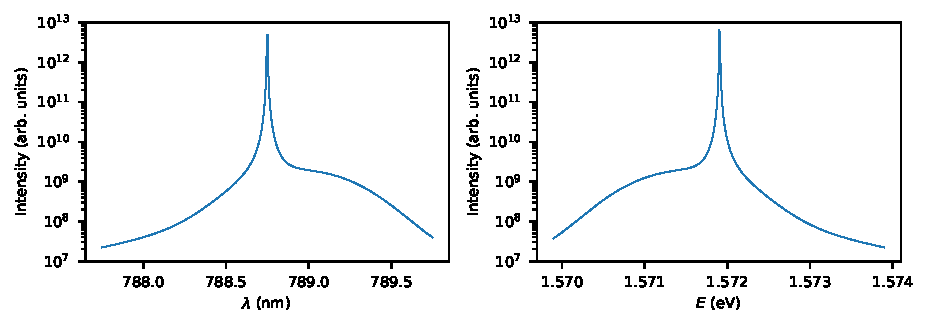
\includegraphics{figures/fabry-perot/plots/quantum_dot_emission_wavelength_energy}
	\caption[Simulated exciton emission of a GaAs quantum dot]{Simulated exciton emission of a GaAs quantum dot plotted dependant on the wavelength $\lambda$ and the Energy $E$.
	The parameters can be found in table~\ref{tab:quantum-dot-emission}.}
	\label{fig:quantumdotemissionwavelengthenergy}
\end{figure}


Dot-Spectra in far field is (TEM$_{00}$).


\section{Adiabatic Rapid Passage}

